\subsection{Introduction to the Choicely voting platform}
    % what does the company do? 
    Choicely \footnote{\url{http://choicely.com/}} is a voting platform developed by a Finnish startup, Lovented Ltd, since 2014. The software provides the possibility for users to engage in interesting contests by voting on their favorite contender. The platform has already hosted numerous contests in various fields, such as beauty pageants, public polls, design contests, sport events among many others. The customer base of the firm consist of mainly Finnish broadcasters, publishers and advertisers. However, the last year has brought numerous users and customers from all around the world.
    
    % what are the contests like, what kind of configuration settings are available?
    % The contests in the platform are created by users or brands. 
    Contests can be of multiple types: ... % TODO ask Kaius 
    
    % voting options
    Various voting options are available for contests. The author of the contest has the choice of setting a limit on how many votes users can spend on individual participants or the whole contest in overall. For instance, if the maximum votes in the contest is set to 1, users can give exactly one vote on exactly one participant. Configuration settings allow infinite votes as well. Removing votes is possible, if the author has decided to enable this possibility. Votes cannot be modified after the contest has ended.
    
    % free-silver-gold votes
    On top of the regular free votes, contest authors may allow users to earn more votes (called "silver votes") by sharing the contest on social media or by watching advertisements. Furthermore, authors can allow users to purchase more votes (called "star votes" or "gold votes") with exactly the same restriction settings as explained above. Note, however that the configuration for the three vote types are distinct for every contest. This means that the limitation on free/silver/star votes may differ for individual participants as well as the whole contest. 

    % how can one reach a contest in the platform?
    Contests can be accessed through multiple interfaces (Figure \ref{choicely_platforms}). Naturally, the company's webpage provides a convenient way to create, browse and participate in contests. Choicely also has free mobile applications available on Android and iOS devices, that can be installed through the Google Play \footnote{\url{https://play.google.com/store/apps/details?id=com.choicely.android}} and the iOS App Store \footnote{\url{https://itunes.apple.com/fi/app/choicely/id1158798364}} on the devices. Finally, the company offers a web widget, which can be embedded as a framework in any webpage easily. The last option is often used by many of Choicely's customers, because it provides a convenient way to embed rich content in their own web pages. 
    
    % what do users have to do to participate? 
    Majority of the contests require users to have a user profile in the Choicely platform. Optionally, profiles can be created through a regular sign-up process, where users register and pick a password for their authentication. When users choose this kind of registration, their e-mail addresses are confirmed through a verification link sent to their inbox, so that their identity is confirmed. Each user profile contains the features listed in Table \ref{user_profile_fields}. 

    \begin {table}[]
        \centering
        \begin{tabular}{l|l}
            \textbf{Field}              & \textbf{Type} \\
            \hline
            Full name                   & Free text \\
            Profile picture             & Image \\ 
            Cover image                 & Image \\
            Gender                      & Male/Female/Other/Not specified \\
            Location                    & Country, state and city \\
            Birthday                    & Datetime \\ 
            Age group                   & 0-17/18-24/25-34/35-44/45-54/55-64/65+ \\
            Introduction/Bio            & Free text
        \end{tabular}
        \caption{The pruning rules used for preprocessing the data.}
        \label{user_profile_fields}
    \end{table}

    % what is the connection between contests and users? How do the participate?
    Users may vote and participate in their own contests if they like. Users may participate in arbitrary number of contests from three platforms: the two most popular mobile platforms (iOS and Android) and the web interface (Figure \ref{choicely_platforms}). 
    
    \begin{figure}[h] 
        \begin{center}
            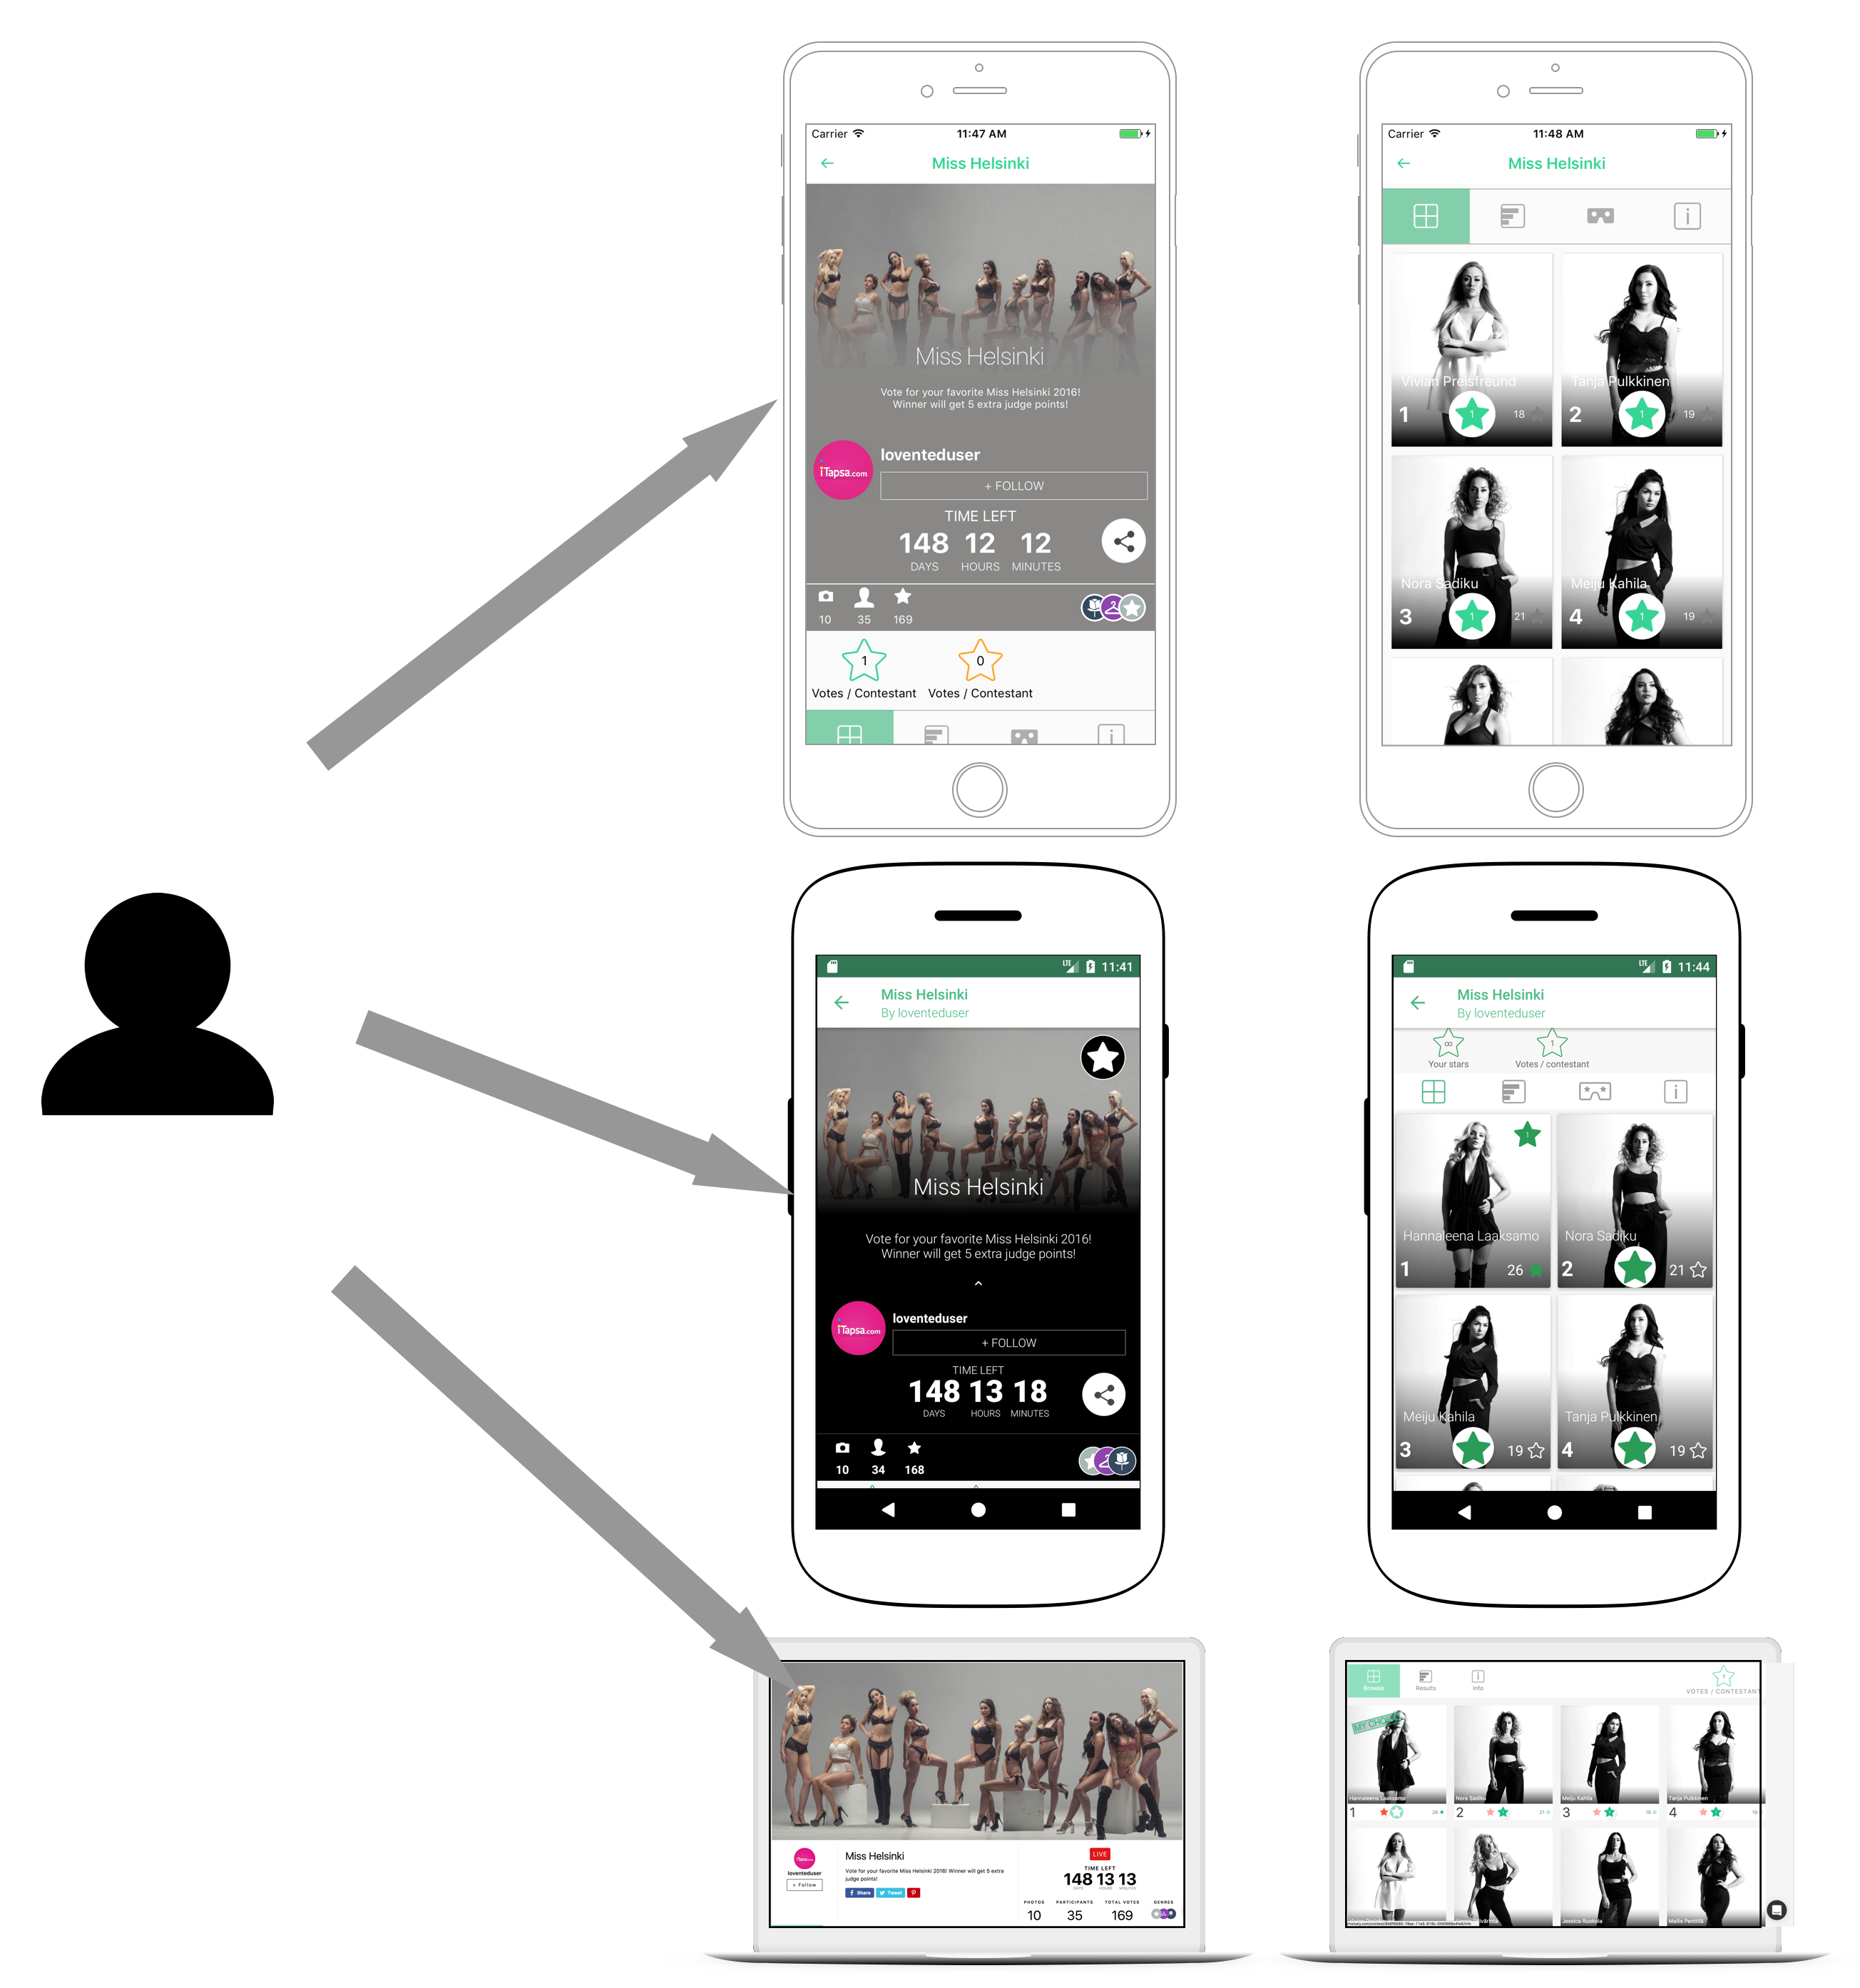
\includegraphics[width=0.6\textwidth]{images/choicely_platforms.png}
            \caption{Users can vote in contests through three interfaces: iOS devices, Android devices and web.}
            \label{choicely_platforms}
        \end{center}
    \end{figure}

    % what kind of data is generated?
    The available data is two-folded: each user has a user profile, which contains basic demographic information about the user (gender and location), while contests have a number of participants with arbitrary number of votes that the users have spent on them. The vote changes for the contests are stored as transactions. This means that the database contains not the final results of the voting, but rather the changes what users made while using the software. This way it is possible to analyze the votes over time and to look at changes individually. For instance, it is possible to tell if a user has removed his/her votes from participant A and moved them to participant B. Furthermore, this way of data representation to restore or simulate any previous state of the contest, in case it would be needed.

    % how does the data look like and how can it be retrieved?
    The data is structured in nature and is stored in a... The data can be accessed via...

    %  why is it important to analyze this kind of data and what can we learn from it? 
    There is a need to analyze this data, because...
    
\subsection{Research setting}
    % why is the data analysis relevant from scientific research point of view?
    Performing scientific research on such data is interesting for multiple reasons. To begin with, at the beginning of the research Choicely does not utilize data analysis tools to gain better understanding on the collected data. It is in the interest of the company and its customers to better understand what kind of audience was engaged in the past, what kind of content is more (or less) successful, what the tendencies in user behavior are. As a result, the introduction of data visualization and analysis tools at the company will greatly enhance business value of the firm and provide deeper understanding on the domain as well as the user base.   
    
    % how is Choicely different than other social networks or any other repository of user data?
    Secondly, Choicely can be looked at as a social network, because some of the platform uploaded to the platform is generated by users. Users also have the possibility to express their appreciation or support towards some contest participants by spending votes on them. Similarly to social networking sites, where the "like" feature is often used \cite{jang2015noreciprocity, bakhshi2014faces} this phenomena can be looked at as a way of expressing personal opinion. 
    
    In comparison to most of the currently available social networks, voting platforms like Choicely are observed by the audience differently. On one hand, social media sites usually list posts or images on a feed, where there is theoretically no relation between the posts that follow eachother. On the other hand, contestants in the Choicely platform share similarities as they were nominated for the same contest. Accordingly, there must be some similarity among them as all are subjects of the contest's topic, rules and are competing for the best possible result. 
    
    \begin{figure}[h] 
		\begin{center}
            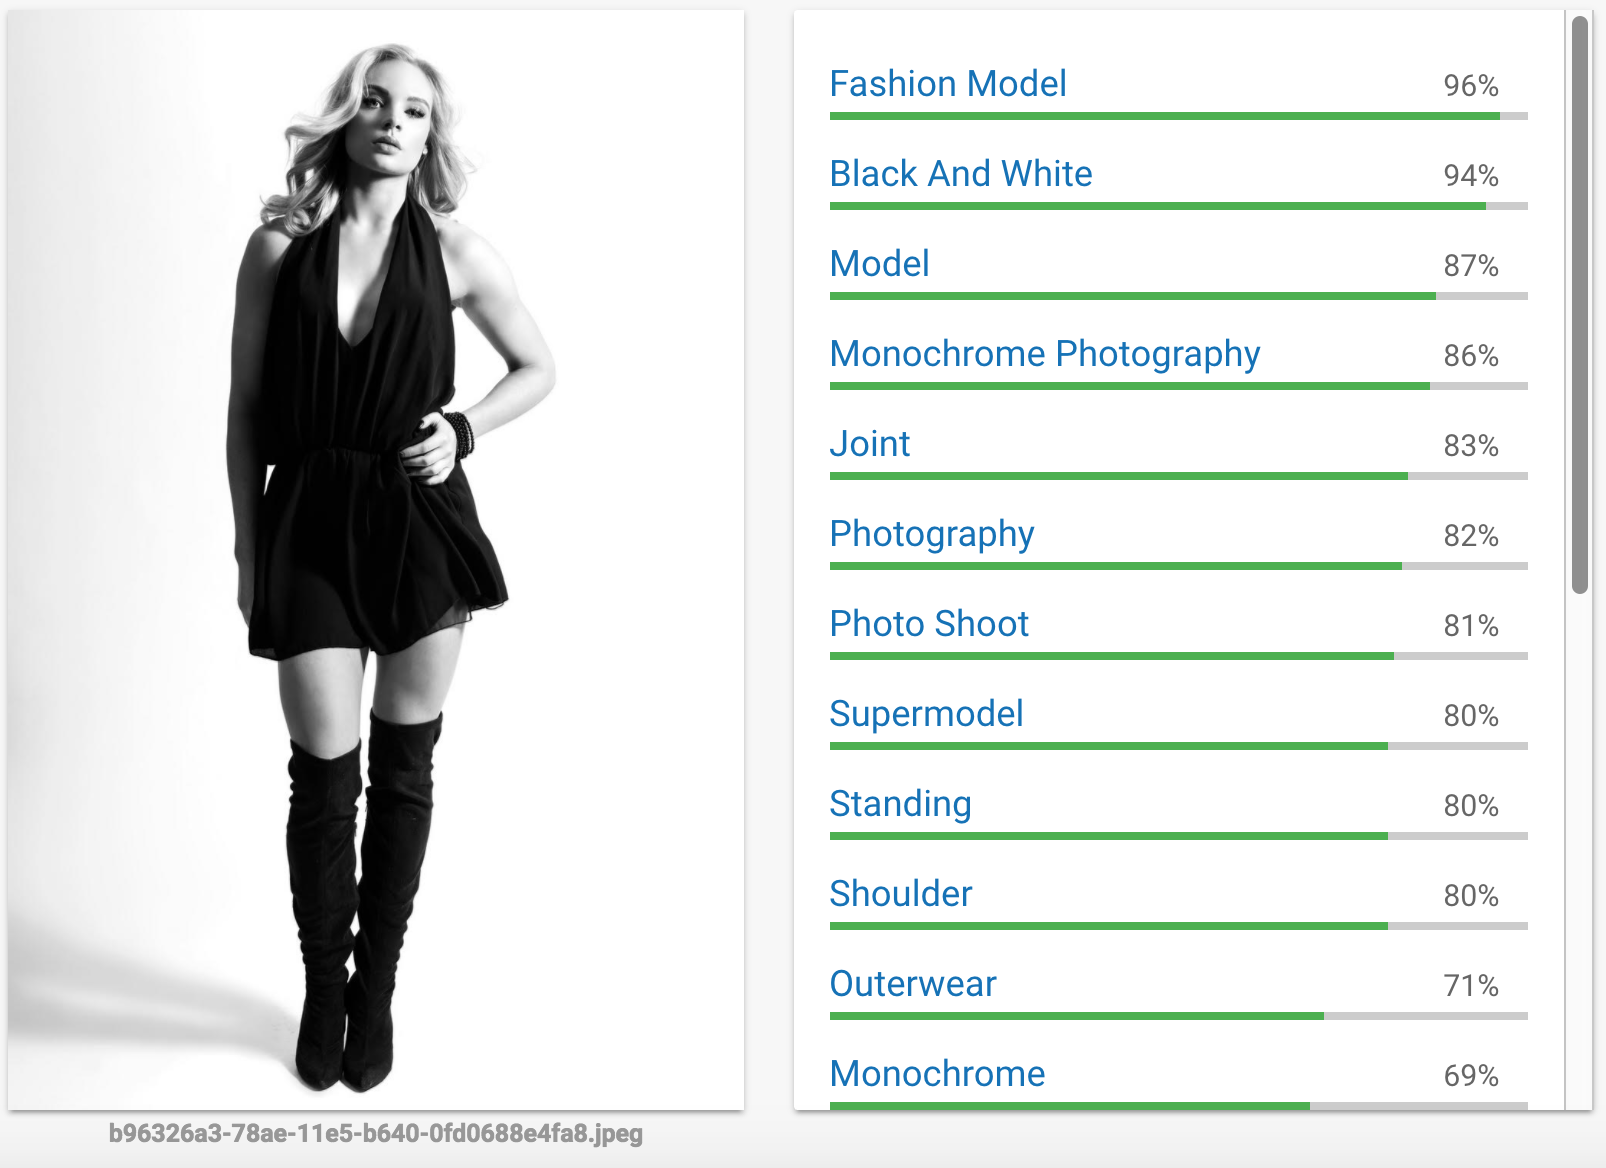
\includegraphics[width=0.8\textwidth]{images/google_vision_labels.png}
            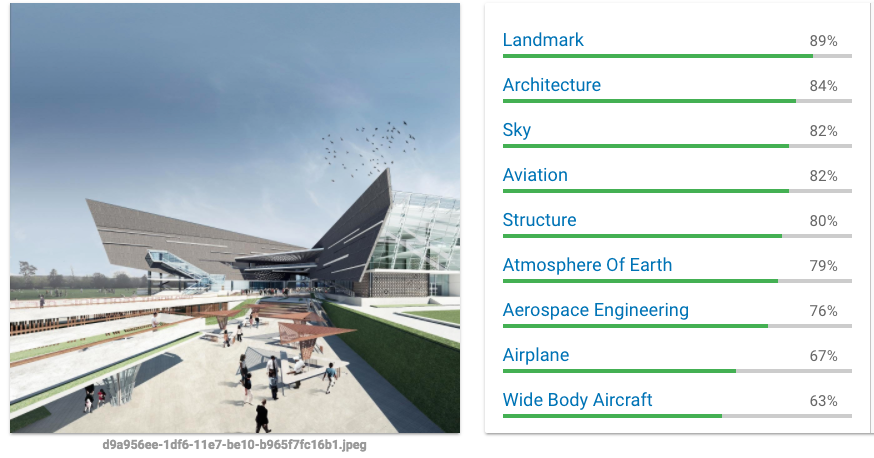
\includegraphics[width=0.8\textwidth]{images/google_vision_labels2.png}
			\caption{The labels identified by the Google Vision API on two of the contest participant's images.}
			\label{google_vision_labels}
		\end{center}
    \end{figure}

    % so what? Why is that important from user point of view
    This slight difference in the content makes a big change in terms of user behavior. The focus moves from "what kind of content I like" to "which piece of content I like the most in comparison to the rest". Consequently, users will scan through some (or optimally all) of the contestants and make unconscious decisions upon whether to give vote(s) on certain contest participant(s). The users express their favour and support towards a subset of contenders, and hence helping them to reach their ultimate goal: winning in the contest. 

    % how can this contribute to user behavior and social media studies? 
    This difference compared to other social networking sites offers a great possibility for research. The potential of identifying what kind of content among different contests individuals like as well as what kind of content similar group of users like, hinders in the data.    

    % how computer vision is going to be utilized? 
    One of the challenges in connecting users with topics of contests is that there is no indication on what the content on the contenders' pictures is. Contest authors only assign categories to the contests to be created, which does not necessarily describe the entrants in the contest. Other researches have successfully utilized computer vision to gather meta data for the uploaded content in image sharing communities \cite{bakhshi2014faces, hu2014we}. Deriving from the success, computer vision is utilized in this research as well to identify labels that appear on the participants' images. For instance, a beauty pageant's entry image may be labelled with meta data, such as "Beauty", "Photo Shoot", "Smile" and "Blonde". Similarly, a design contests entry might have topic labels, such as "Landmark" or "Architecture". Figure \ref{google_vision_labels} displays an example, where the Google Vision API was used as a black box to identify such labels in images, that were extracted from two of Choicely's contests.
    
    % architectural overview
    The current architecture of the Choicely platform is...
    \begin{figure}[h] 
		\begin{center}
            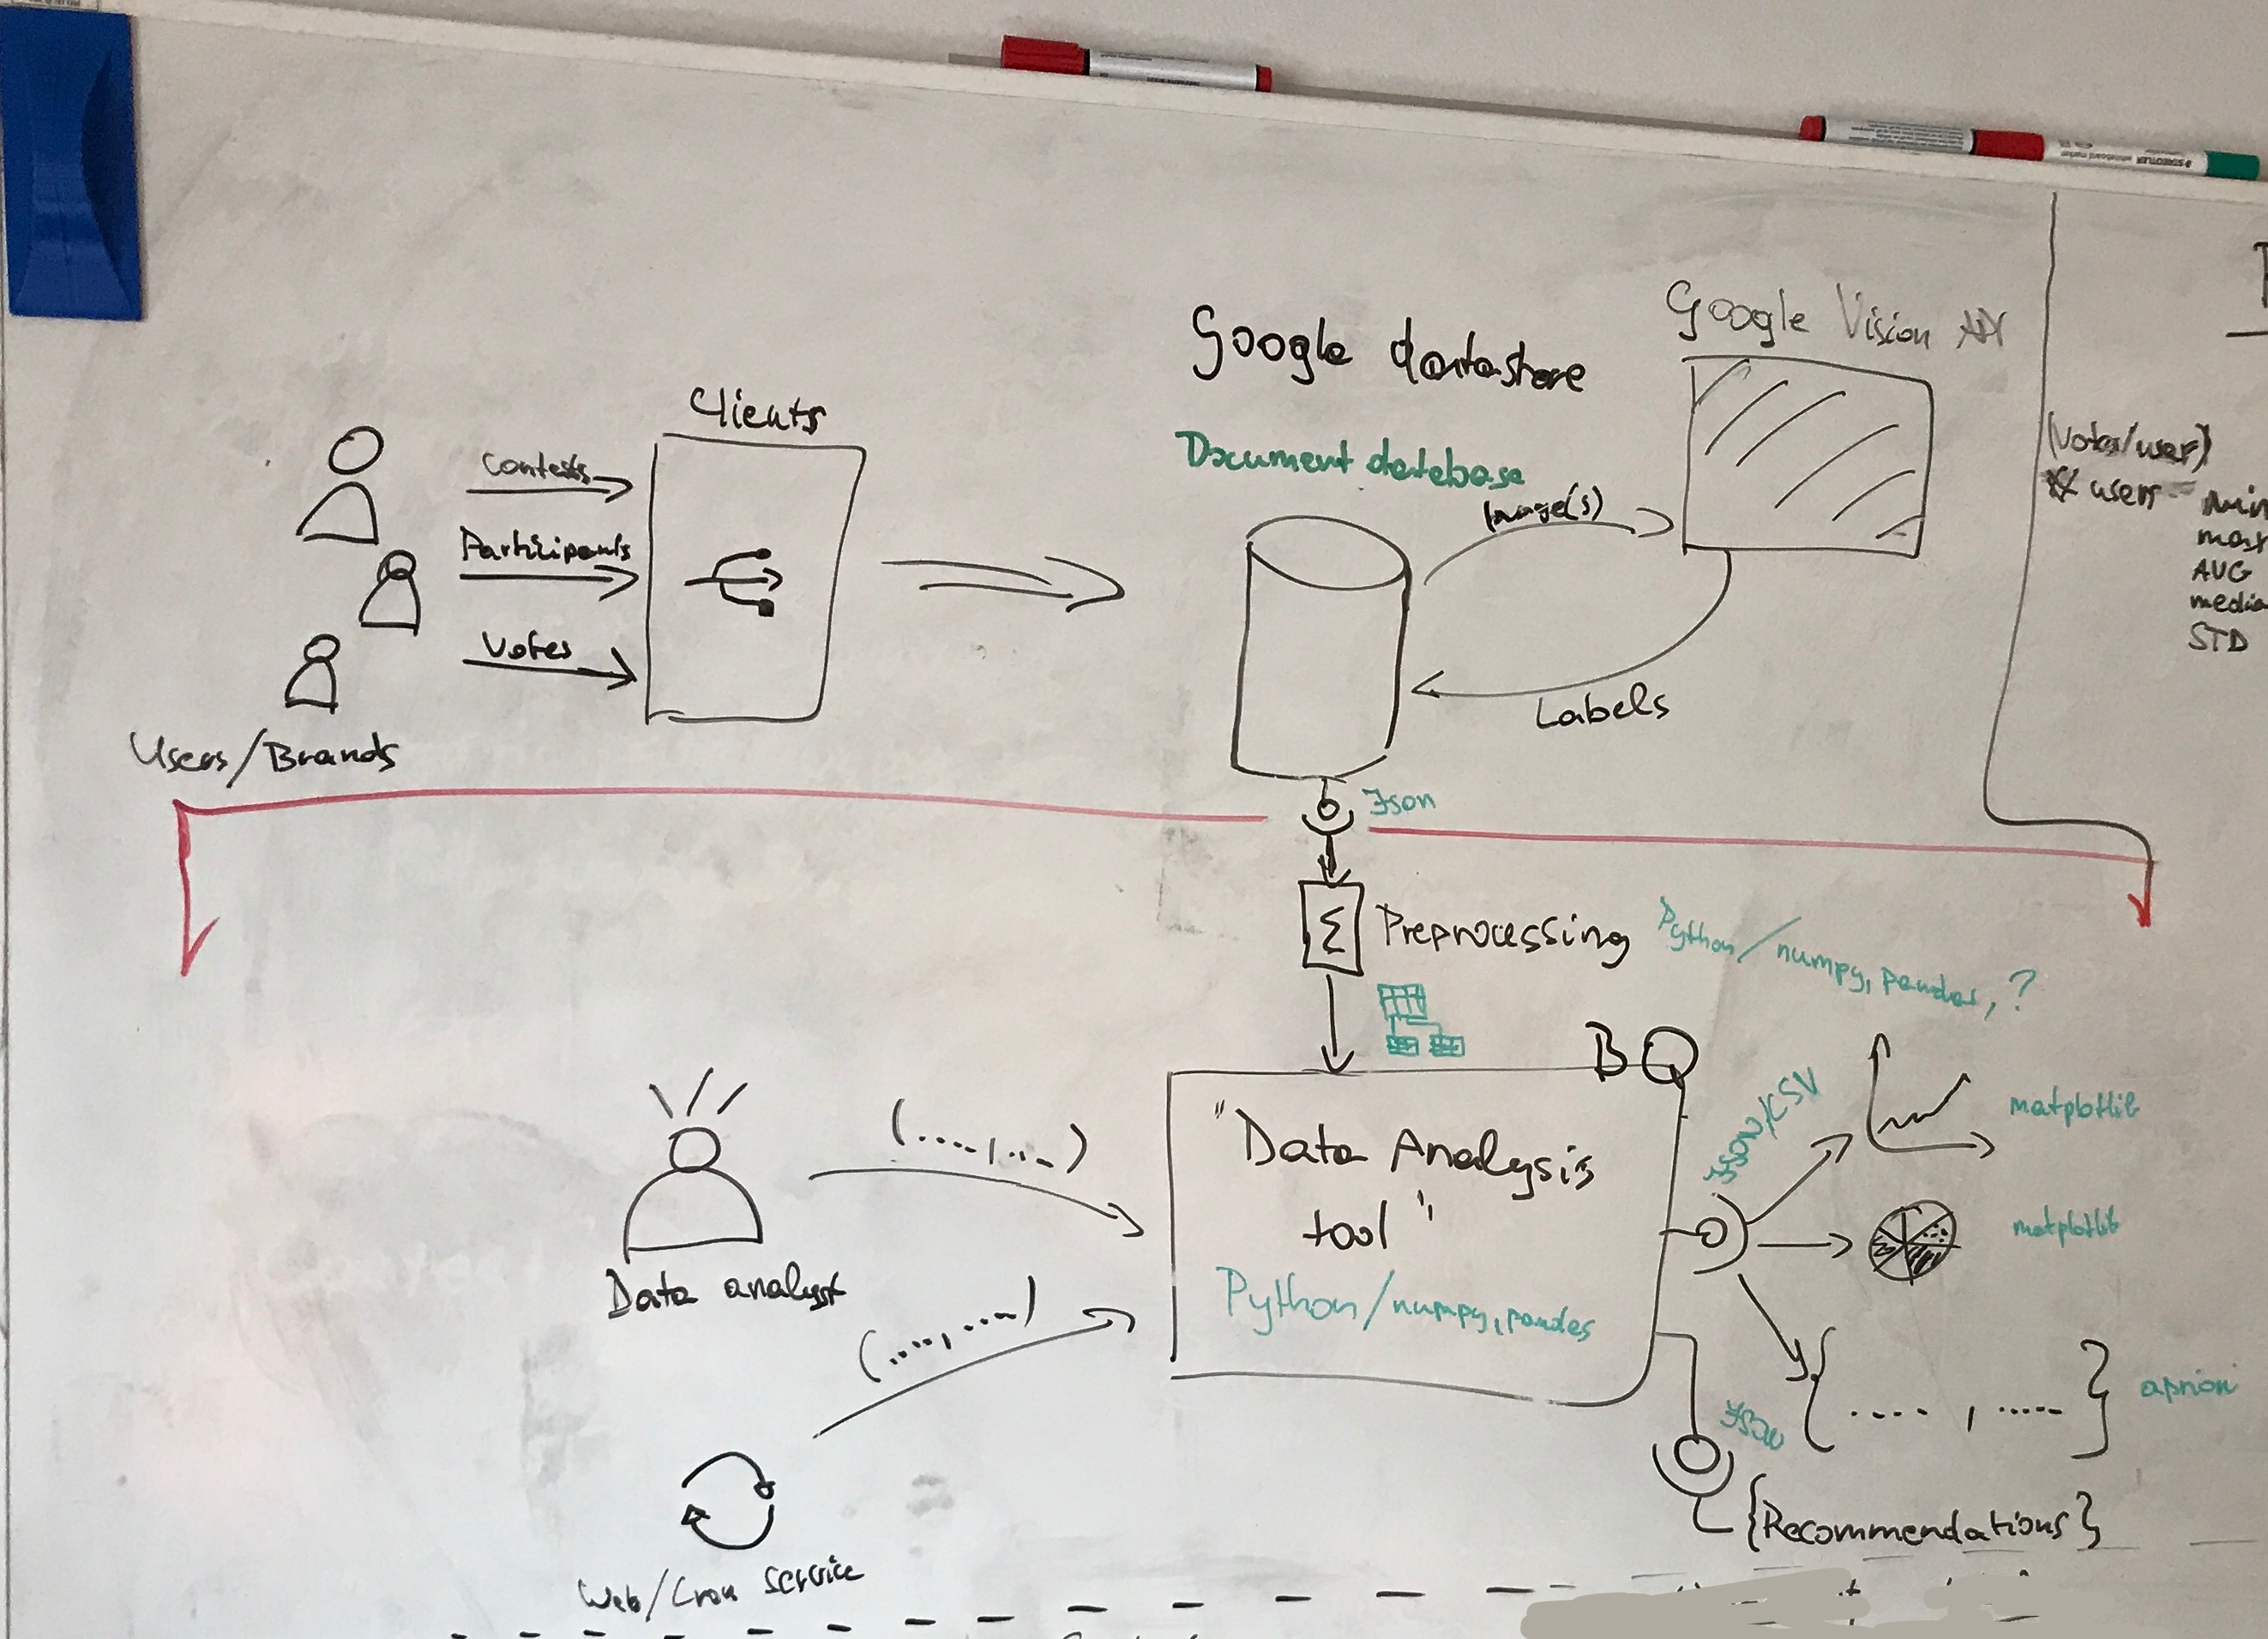
\includegraphics[width=0.8\textwidth]{Images/architecture_whiteboard.jpg}
			\caption{The brief architectural overview of the Choicely platform.}
			\label{choicely_architecture}
		\end{center}
    \end{figure}

    % the structure of the data models
    The structure of the data... 
    \begin{figure}[h] 
		\begin{center}
            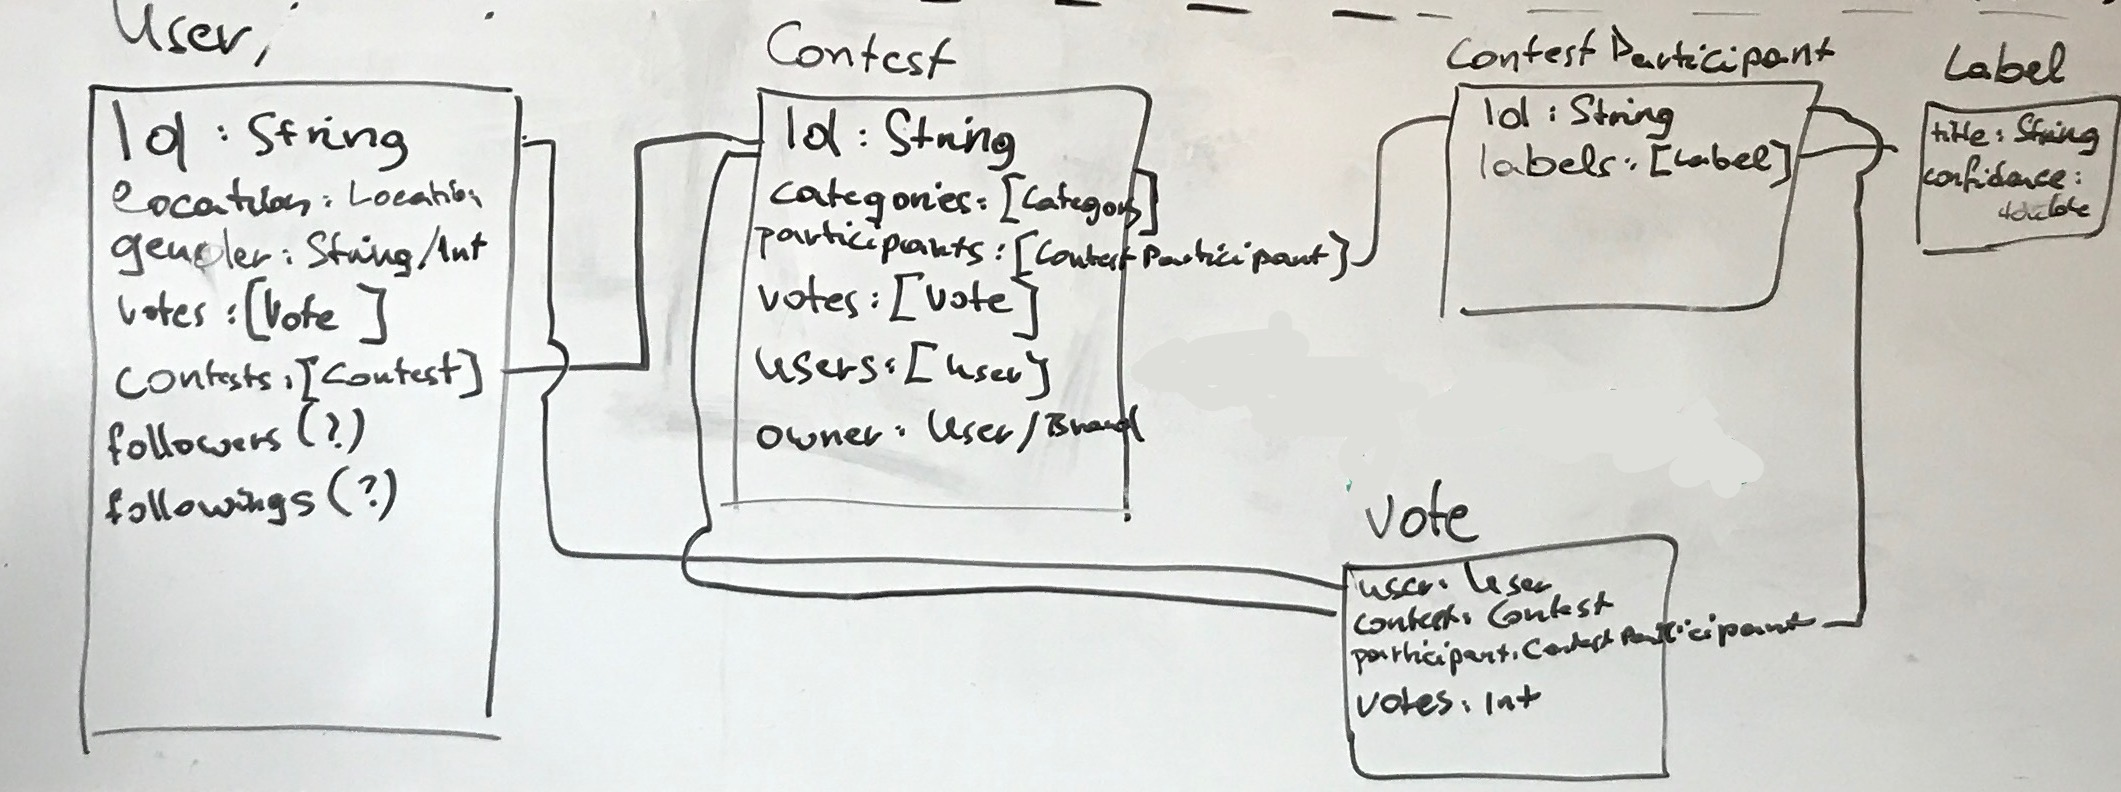
\includegraphics[width=0.8\textwidth]{Images/data_structure_whiteboard.jpg}
			\caption{The structure of the data models of the Choicely platform.}
			\label{choicely_data_models}
		\end{center}
    \end{figure}

\subsection{Methodology} % what kind of methods were chosen? 
    % Exploratory Data Analysis (EDA)
    To grasp on the currently available data, Exploratory Data Analysis (EDA) is utilized as the first step of the research. A comprehensive overview on the data related to the most important entities in the Choicely platform is performed by calculating basic statistical measures and visualizing the data. Such entities are the user profiles, the contests, contest participant and the votes performed by users on the contest participants. The findings of the EDA are then utilized to determine how to prune the data such that the acquired sample is representative, does not contain redundant nor faulty data. The results of the EDA are explained in the next section. 

    % check \cite{socialdiversityongithub} -> Blau index / diversity index: reflects how many different types (such as species) there are in a dataset (a community), and simultaneously takes into account how evenly the basic entities (such as individuals) are distributed among those types.
    
    % what are the decisions behind the choices? 
    % what were the alternatives and why were they rejected? 

\subsection{Results}
    \subsubsection{Exploratory Data Analysis}
    % what are the takeaways of the EDA? % preprocessing
    The EDA has highlighted multiple ways how the data should be pruned in order to ensure the relevance of the data. 

    \subsubsection{Preprocessing}
    It was identified, that some of the data cannot be used for the purposes of this study and the results will be more representative, if some of the data is pruned. Hence, the following rules were applied to prune the data:

    \begin {table}[]
        \centering
        \begin{tabular}{l|l}
            \textbf{Entity}              & \textbf{Pruning rule} \\
            \hline
            \textbf{Contest}             & Unique voters < 100 or Unique voters == null or Contest participants < 2 \\
            \textbf{ContestParticipant}  & Number of labels < 0 
        \end{tabular}
        \caption{The pruning rules used for preprocessing the data.}
        \label{contest_preprocessing_rules}
    \end{table}

    Entities that match any of the rules displayed in Table \ref{preprocessing_rules} are dropped from the analysis. For instance, contests with less than 100 unique voters (users) and images without labels are considered irrelevant, and may bias the results of the study. After applying the preprocessing rules, the dataset is left with 92 contests, 1625 contest participants, 282545 votes and XXX unique voters over 10 contest categories. % TODO update occasionally

    \subsubsection{Association analysis}